

\section*{Contents of the dissertation}


\textbf{Introduction} substantiates the relevance of the research, which addresses the robustness and generalization of deep learning models in 3D medical image segmentation under domain shift. It formulates the main goals and objectives of the dissertation, outlines the applied research methodology, highlights the scientific novelty of the proposed domain adaptation approaches and evaluation frameworks, and emphasizes the theoretical and practical significance of the results. The section concludes by stating the key contributions and propositions submitted for defense, approbation and reliability of the work.


% %%%%%%%%%%%%%%% CHAPTER 1 %%%%%%%%%%%%%%%


The first chapter, \textbf{Domain Shift Anatomy}, focuses on understanding how domain shifts impact CNNs for medical image segmentation, particularly in MRI. This chapter studies the vulnerability of CNN layers to domain shift and proposes an adaptive fine-tuning approach to mitigate its negative effects.

We begin by evaluating a supervised DA scenario, where the training and target domains represent the same content (e.g., brain MRI), but differ due to acquisition settings and scanner vendors. For this study, we employ the CC359 dataset~\cite{cc359}, and the segmentation task is performed using a U-Net model~\cite{unet}. An initial set of experiments demonstrates that fine-tuning only the first layers of a CNN (closest to the input) leads to better adaptation results compared to full-network or last-layer tuning. This suggests that the low-level feature maps, which capture basic visual patterns like edges and textures, are the most sensitive to acquisition variability.
%We trained the model on the source domain and adapted to the target domain in a few-shot scenario, using 1 to 4 annotated target image slices.

We then introduce SpotTUnet, a method that automatically identifies which layers to fine-tune based on a learnable layer selection policy. Formally, the policy mechanism could be stated as follows. We compute the output for the $l$-th network layer as


\begin{equation}
	x_l = I_l ( x ) F_l ( x_{l-1} ) + (1 - I_l ( x )) \tilde{F}_l ( x_{l-1} ),
\end{equation}

\noindent
where $F_l$ and $\tilde{F}_l$ represent the frozen and fine-tuned versions of the $l$-th block and $I_l(x)$ is the binary indicator derived from the Policy Network’s prediction.

Policy Network is trained concurrently with the fine-tuning of the segmentation network. During each iteration, Policy Network makes ``soft'' predictions for each block, which we binarize (into $I_l(x)$) to determine whether to use the frozen or fine-tuned block. To ensure gradient flow through the binary decision-making process, we employ the Gumbel-Softmax trick~\cite{jang2017categorical} in the following way.% This approach allows gradients to be propagated through the binary indicator $I_l(x)$, enabling end-to-end training.

%The binary indicator $I_l(x) \in \{0, 1\}$ represents a discrete decision, which is inherently non-differentiable. To enable gradient-based optimization, we replace this hard decision with a differentiable approximation based on the Gumbel–Softmax (also known as the Concrete) distribution.

Let the Policy Network produce for each block $l$ a pair of unnormalized logits $\mathbf{z}_l(x) = [z_{l,0}(x),\, z_{l,1}(x)],$ corresponding to the probabilities of using the frozen ($I_l=0$) or fine-tuned ($I_l=1$) version of the block. The categorical sampling operation

\[
I_l(x) \sim \mathrm{Categorical}(\pi_{l,0}, \pi_{l,1}), \quad
\pi_{l,i} = \frac{\exp(z_{l,i})}{\sum_{j} \exp(z_{l,j})},
\]

\noindent
is replaced by a continuous relaxation:

\begin{equation}
	\tilde{I}_l(x) =
	\frac{
		\exp\!\left((z_{l,1} + g_1)/\tau\right)
	}{
		\exp\!\left((z_{l,0} + g_0)/\tau\right) +
		\exp\!\left((z_{l,1} + g_1)/\tau\right)
	},
	\label{eq:gumbelsoftmax}
\end{equation}

\noindent
where $g_0, g_1$ are independent samples from the $\mathrm{Gumbel}(0,1)$ distribution,

\[ g = -\log(-\log u), \quad u \sim \mathrm{Uniform}(0,1), \]

\noindent
and $\tau > 0$ is a temperature parameter controlling the smoothness of the approximation. In the limit $\tau \to 0$, the expression in~\eqref{eq:gumbelsoftmax} approaches a hard binary decision, while for higher $\tau$ values, it yields a smooth, differentiable interpolation between the two options. %During training, $\tau$ is typically annealed towards zero to gradually enforce discreteness while preserving gradient flow in the early stages of optimization.

%In our framework, we define the effective indicator as
%
%\[
%I_l(x) =
%\begin{cases}
%	1, & \tilde{I}_l(x) > 0.5, \\
%	0, & \text{otherwise},
%\end{cases}
%\quad \text{(forward pass)}
%\]

%\noindent
%while in the backward pass, gradients are propagated through the continuous relaxation $\tilde{I}_l(x)$. This approach ensures that the Policy Network receives meaningful gradients even though the decision process is discrete at inference time.
In the backward pass, gradients are propagated through the continuous relaxation $\tilde{I}_l(x)$. This approach ensures that the Policy Network receives meaningful gradients even though the decision process is discrete at inference time.


In addition to the standard segmentation loss ($\mathcal{L}_{segm}$), we introduce a regularization term to control the number of blocks that are fine-tuned:

\begin{equation}
	\mathcal{L} = \mathcal{L}_{segm} + \lambda \sum_{l=1}^N \left( 1 - I_l (x) \right).
\end{equation}

We present SpotTUnet architecture schematically in Figure~\ref{fig:spottune_seg} and the impact of proposed regularization on the sensitivity profile in Figure~\ref{fig:layerswise_template}.

\begin{landscape}
	\begin{figure}[p]
		\centering
		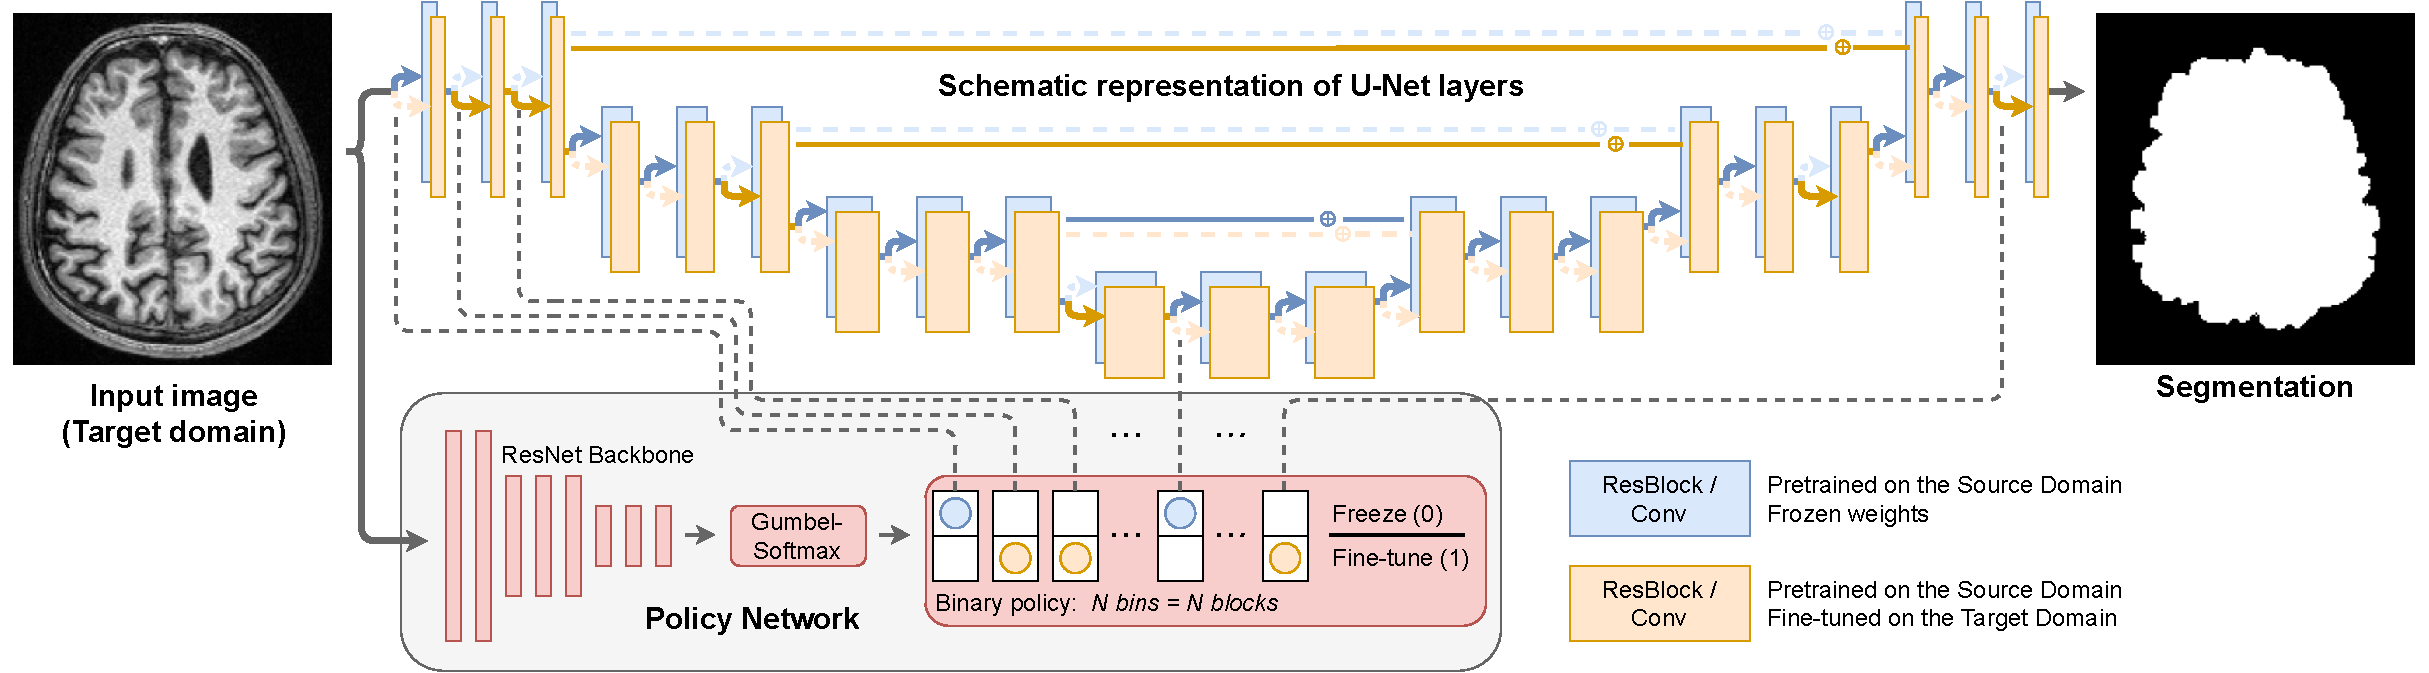
\includegraphics[width=\linewidth]{Dissertation/Figures/2_mri/spottune_seg.pdf}
		\caption{SpotTUnet architecture for the supervised DA in medical image segmentation.}% The U-Net backbone is pretrained on the source domain. This network is frozen (blue blocks) and has a copy (orange blocks) that is fine-tuned on the target domain. The policy network is simultaneously trained on the target domain to output binary decisions for each pair of blocks from the segmentation networks: use the frozen block (blue) vs. use the fine-tuned block (orange).}
	\label{fig:spottune_seg}
\end{figure}
\end{landscape}

\begin{landscape}
	\begin{figure}[p]
		\centering
		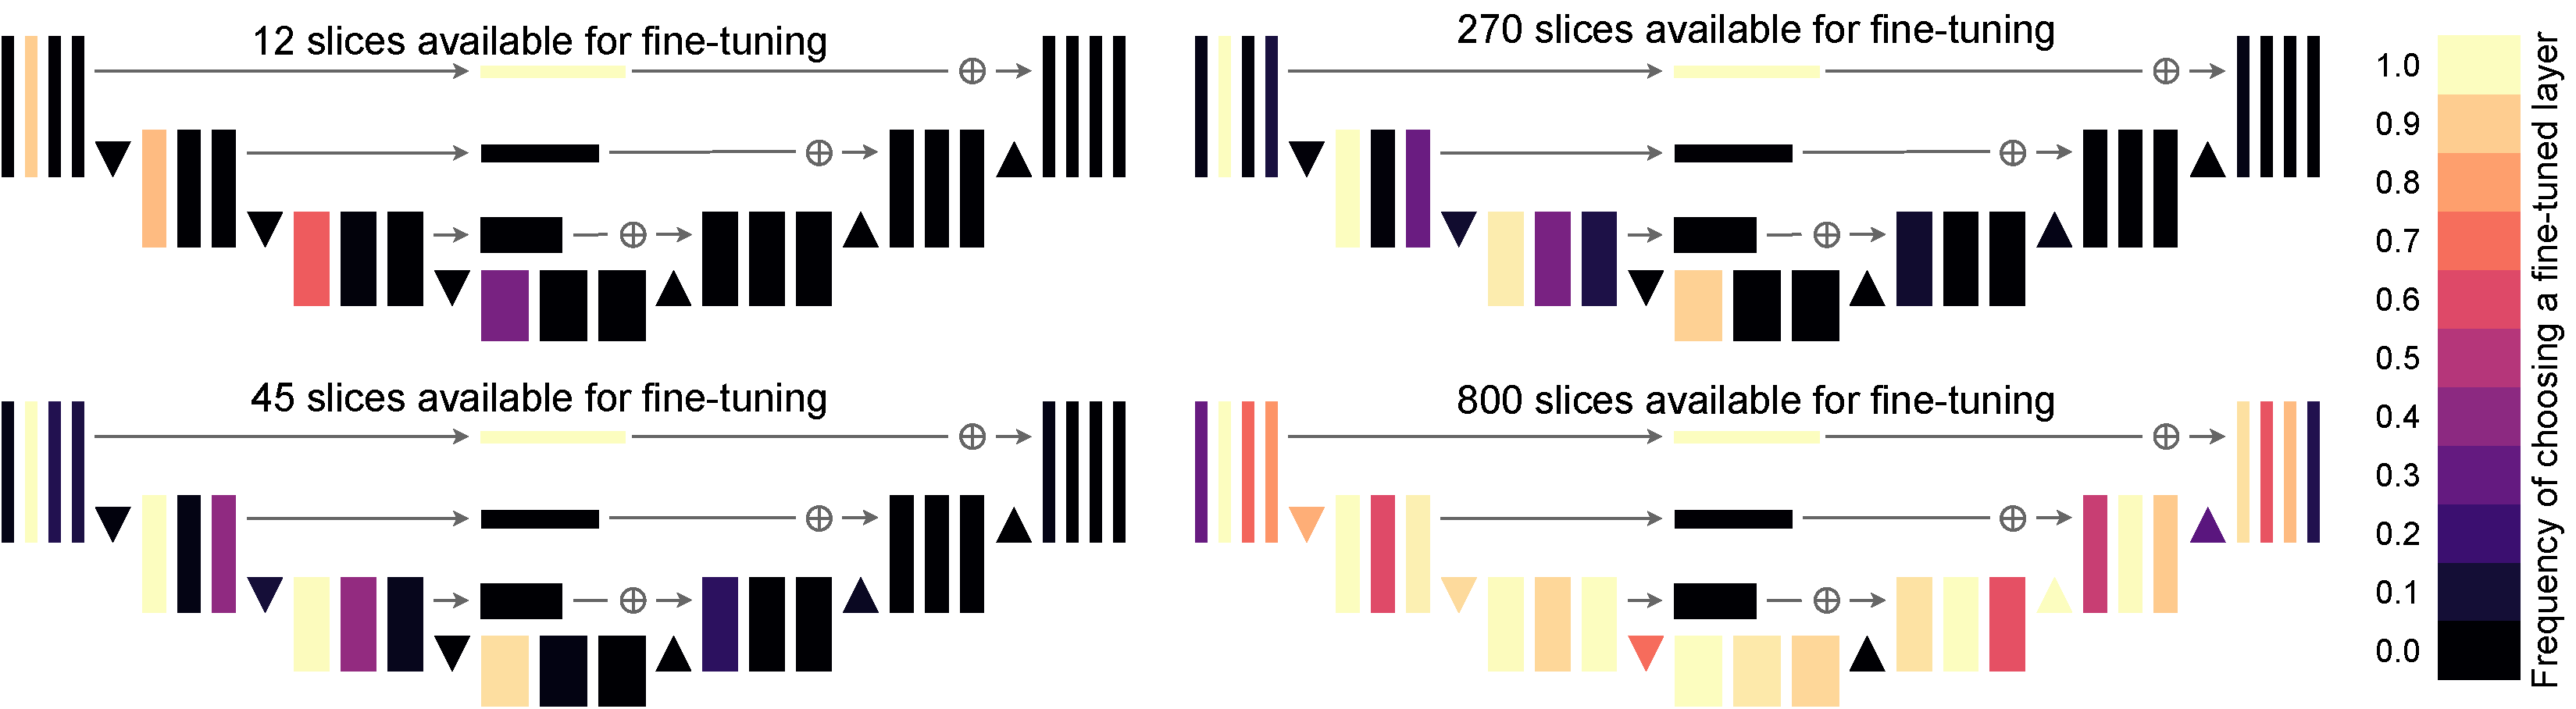
\includegraphics[width=\linewidth]{Dissertation/Figures/2_mri/layerwise_template.pdf}
		\caption{Visualization of SpotTUnet's learned policy for different amounts of available target slices: 12 (upper-left), 45 (bottom-left), 270 (upper-right), and 800 (bottom-right). Colored blocks correspond to residual blocks, with triangular blocks indicating convolutions that perform $\times 2$ up- or down-sampling.}
		\label{fig:layerswise_template}
	\end{figure}
\end{landscape}

The $\mathbb{L}_1$ regularization term allows minimizing the total number of fine-tuned blocks, leading to a sparser, more deterministic and interpretable policy. As a result, SpotTUnet not only significantly outperforms other layer selection heuristics but also enables interpretable analysis of domain shift effects inside the model. Figure~\ref{fig:layerswise_template} illustrates a layer-wise shift sensitivity profile, highlighting the layers most affected by the domain differences.

The results of this chapter lay the conceptual foundation for later methods introduced in the thesis: F-Consistency, which leverages SpotTUnet’s layer selection for adaptation in CT images, and IHF, which builds on the finding of early-layer sensitivity by extracting domain-specific features directly from the input image.


% %%%%%%%%%%%%%%% CHAPTER 2 %%%%%%%%%%%%%%%


The second chapter, \textbf{Mitigating Domain Shift from CT Reconstruction Kernels}, presents a study of a clinically significant source of domain shift in computed tomography (CT) images: variation in image reconstruction kernels. These kernels, integral to the Filtered Back-Projection (FBP) process~\cite{schofield2020image}, determine image texture, smoothness, and noise characteristics~\cite{schaller2003spatial}. While the anatomical content of such images remains unchanged, the variation in appearance can cause a severe degradation in segmentation performance of deep neural networks~\cite{choe2019deep,lee2019ct}.

To quantitatively investigate the problem, we collected datasets of paired CT reconstructions~\cite{morozov2020mosmeddata,tsai2021rsna}, i.e., multiple versions of the same scan reconstructed with different kernels. Surprisingly, despite anatomical identity, models trained on one reconstruction style often fail on the other, achieving an average Dice score of only 0.46.

To address this issue, we firstly introduced Filtered Back-Projection Augmentation (FBPAug) -- a novel knowledge-driven augmentation technique rooted in the mathematical model of CT image formation. FBPAug simulates domain shifts by introducing kernel-like transformations directly in the sinogram domain. We derive it by simulating the original FBP process.

FBP consists of two sequential operations: generation of filtered projections and image reconstruction by the Back-Projection (BP) operator. Projections of attenuation map have to be filtered before using them as an input of the Back-Projection operator. The ideal filter in a continuous noiseless case is the ramp filter. Fourier transform of the ramp filter $\kappa(t)$ is $\mathcal{F}[\kappa(t)](w) = |w|$.

The image $I(x, y)$ can be derived as follows:
\begin{equation}
	\label{eqn:main_eq}
	I(x, y) = \text{FBP}(p_\theta(t)) = \text{BP}(p_\theta(t) * \kappa(t)),
\end{equation}
where $*$ is a convolution operator and $t = t(x,y) = x\cos\theta + y\sin\theta$.% and $\kappa(t)$ is the aforementioned ramp filter.

Assume that a set of filtered-projections $p_{\theta}(t)$ available at angles $\theta_1, \theta_2, ..., \theta_n$, such that $\theta_i = \theta_{i - 1} + \Delta\theta,~i=\overline{2,n}$ and $\Delta\theta = \pi / n$. In that case, BP operator transforms a function $f_\theta(t) = f(x\cos\theta + y\sin\theta)$ as follows:
\[
BP(f_\theta(t))(x, y) = \frac{\Delta\theta}{2\pi}\sum\limits_{i=1}^n f_{\theta_i}(x\cos\theta_i + y\sin\theta_i) = \frac{1}{2n}\sum\limits_{i=1}^n f_{\theta_i}(x\cos\theta_i + y\sin\theta_i)
\]

In fact, $\kappa(t)$ that appears in (\ref{eqn:main_eq}) is a generalized function and cannot be expressed as an ordinary function because the integral of $|w|$ in inverse Fourier transform does not converge. However, we utilize the convolution theorem that states that $\mathcal{F}(f*g) = \mathcal{F}(f)\cdot\mathcal{F}(g)$. And after that we can use the fact that the BP operator is a finite weighted sum and Fourier transform is a linear operator as follows:
\[
\mathcal{F}^{-1}\mathcal{F}[I(x, y)] = \mathcal{F}^{-1}\mathcal{F}[\text{BP}(p_\theta * \kappa)] = \text{BP}(\mathcal{F}^{-1}\mathcal{F}[p_\theta * \kappa]) = \text{BP}(\mathcal{F}^{-1}\{\mathcal{F}[p_\theta]\cdot|w|\}),\]
\[I(x, y) = \text{BP}\left(\mathcal{F}^{-1}\{\mathcal{F}[p_\theta]\cdot|w|\}\right).\]

However, in the real world, CT manufacturers use different filters that enhance or weaken the high or low frequencies of the signal. We propose a family of convolution filters $k_{a,b}$ that allows us to obtain a smooth-filtered image given a sharp-filtered image and vice versa. Fourier transform of the proposed filter is expressed as follows:
\[\mathcal{F}[k_{a,b}](w) = \mathcal{F}[\kappa](w)(1 + a \mathcal{F}[\kappa](w)^b) = |w|(1 + a|w|^b).\]

Thus, given a CT image $I$ obtained from a set of projections using one kernel, we can simulate the usage of another kernel as follows:
\[\hat{I}(x, y) = \text{BP}\left(\mathcal{F}^{-1}\{\mathcal{F}[\mathcal{R}(I)]\cdot\mathcal{F}[k_{a,b}]\}\right).\]

Here, $\mathcal{R}(I)$ is a Radon transform. Parameters $a$ and $b$ influence the sharpness or smoothness of an output image, with the visual examples given in Figure~\ref{fig:crops}.

\begin{figure}[h]
	\centering
	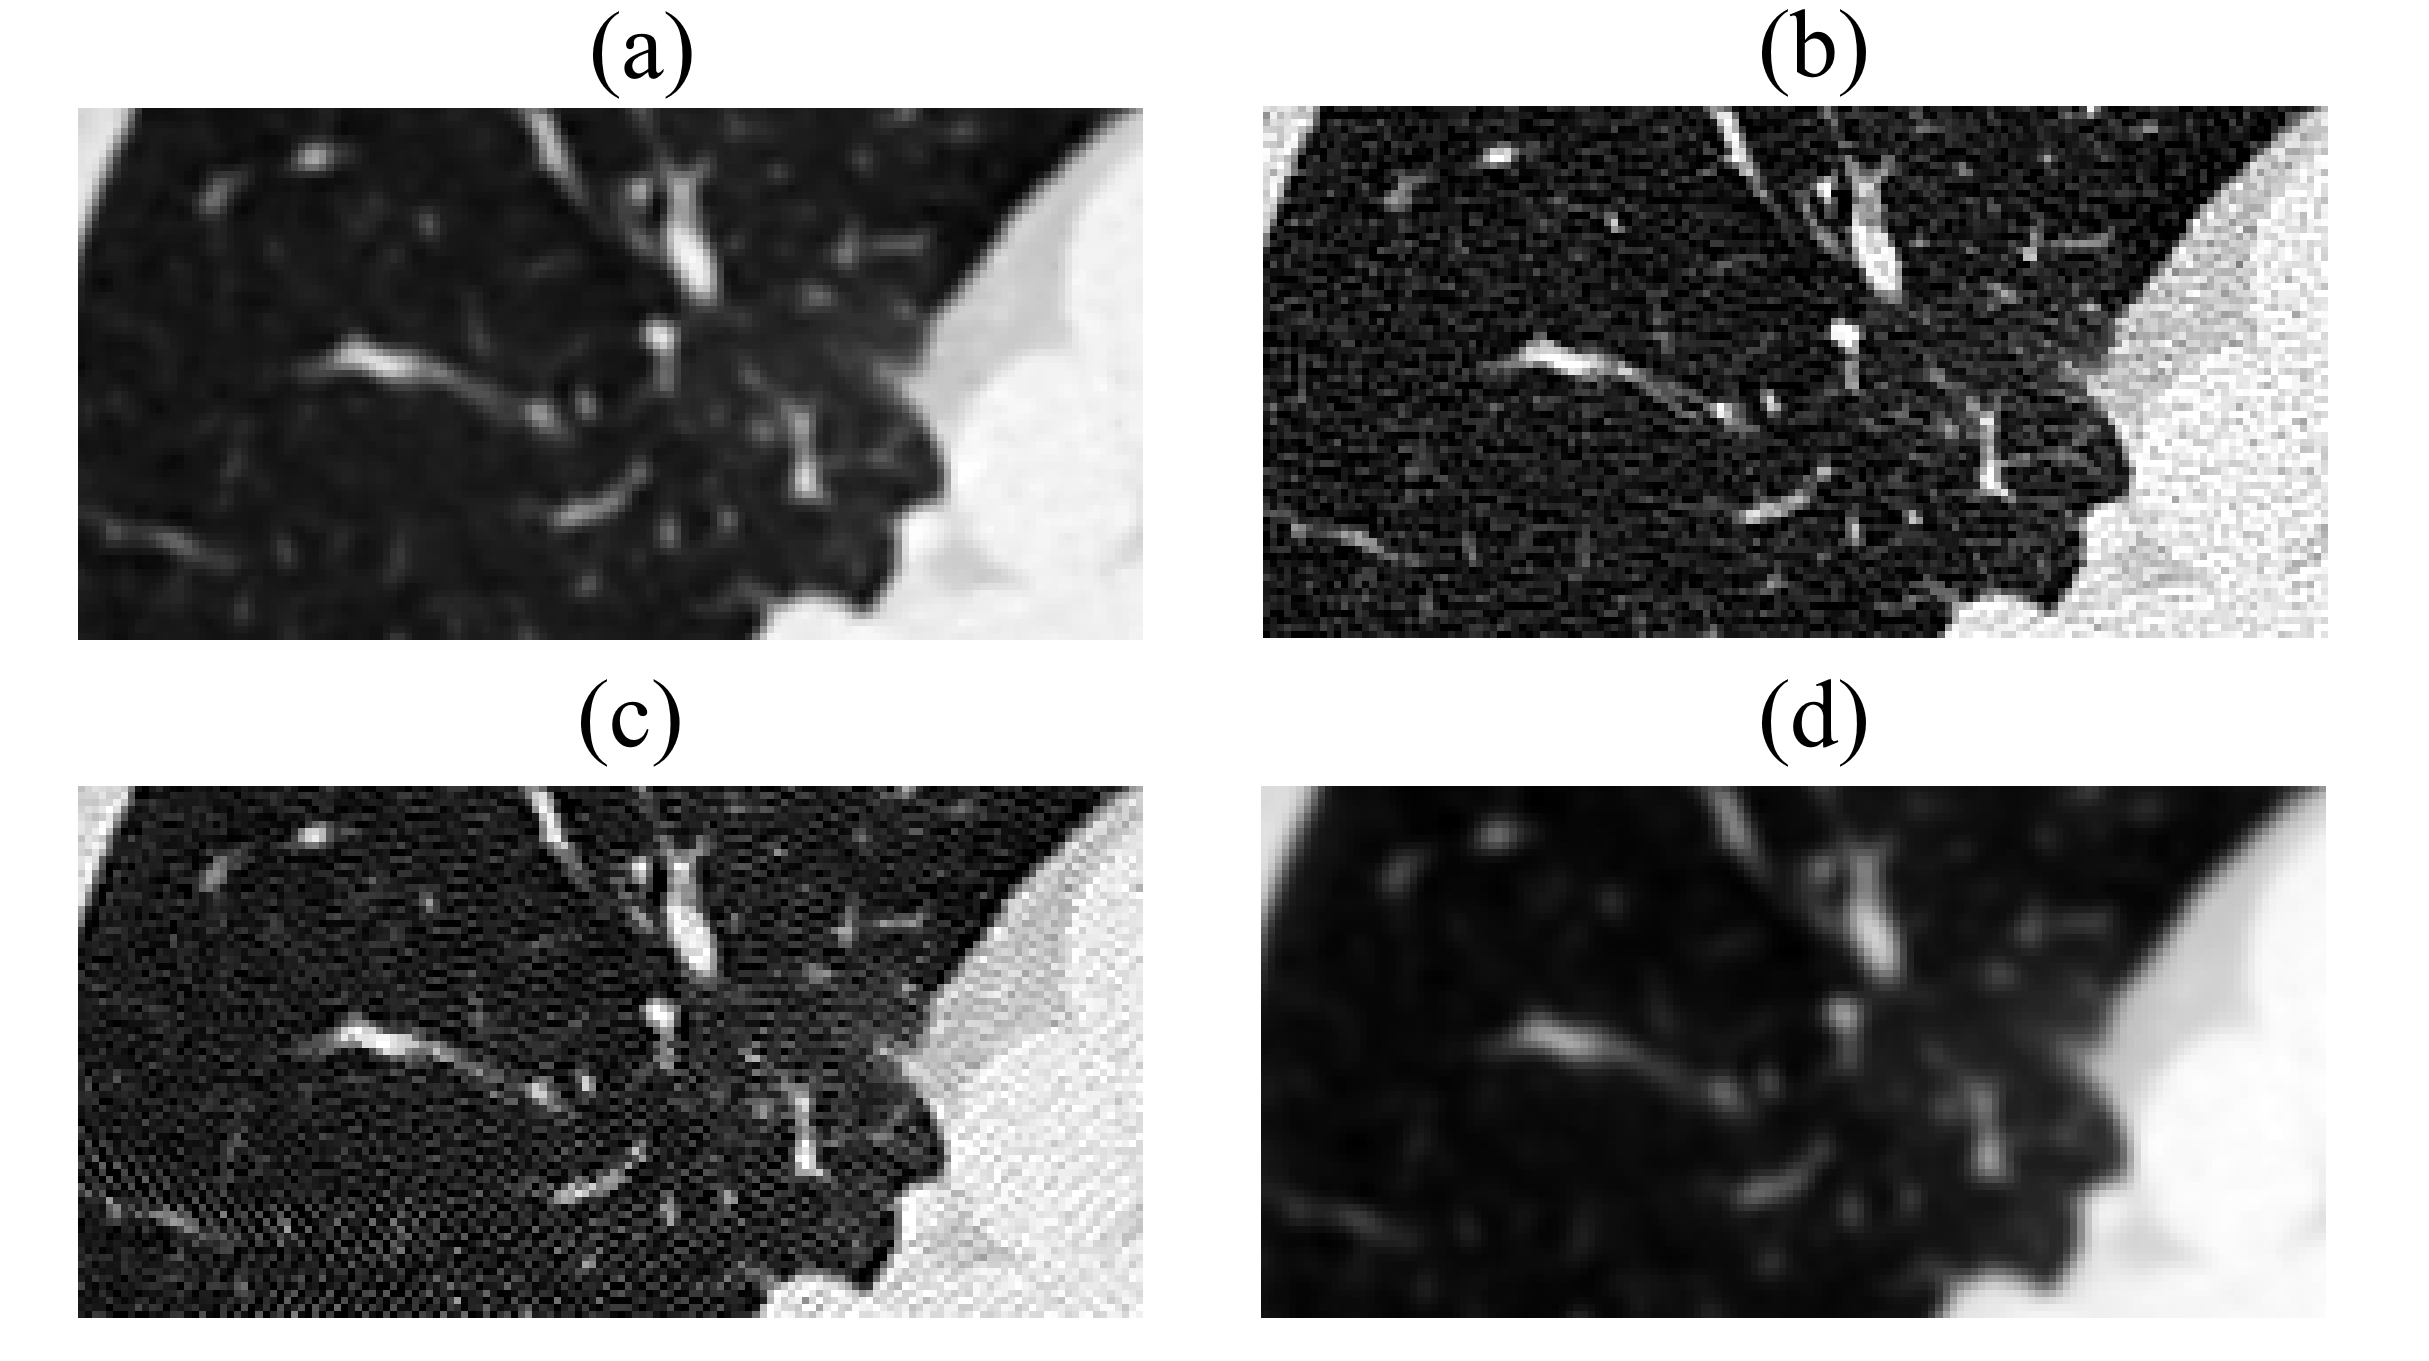
\includegraphics[width=0.95\linewidth]{Dissertation/Figures/3_ct/4crops.png}%[width=7cm][width=7cm]
	\caption{An example of paired CT slices (top row) and the effect of the augmentation by the proposed method (bottom row).} %The top row contains original images: a slice reconstructed either with a smooth kernel (a) or sharp kernel (b). The bottom row shows augmented images: the top-left image processed by FBPAug with parameters $a=30,~b=3$ shifting it from smooth to sharp (c); the top-right image processed by FBPAug with parameters $a=-1,~b=0.7$ from sharp to smooth (d).}
	\label{fig:crops}
\end{figure}

The top row contains original images: a slice reconstructed either with a smooth kernel (a) or sharp kernel (b). The bottom row shows augmented images: the top-left image processed by FBPAug with parameters $a=30,~b=3$ shifting it from smooth to sharp (c); the top-right image processed by FBPAug with parameters $a=-1,~b=0.7$ from sharp to smooth (d).

This method produces synthetic images mimicking the effects of alternate kernels and significantly improves segmentation model generalization. In experiments on COVID-19 segmentation, FBPAug increases cross-kernel consistency from 0.46 to 0.76 in Dice score, almost achieving the level of DA methods that require additional data for fine-tuning (Table~\ref{tab:res_final}).



%\begin{table}[H]
%	\caption{Comparison of all considered methods. The adaptation methods are trained using all training kernel pairs of the Paired-private dataset. F-/P-Cons stand for F-/P-Consistency, where F-Consistency is our proposed method. All results are Dice Scores in the format \textit{mean} $\pm$ \textit{std} calculated from $5$-fold cross-validation. We highlight the best scores in every column in \textbf{bold}.}
%	\begin{adjustwidth}{-\extralength}{0cm}
%		\newcolumntype{C}{>{\centering\arraybackslash}X}
%		\begin{tabularx}{\fulllength}{lCCCCCCC}
%			\toprule
%			
%			& \multirow{2.5}{*}{\textbf{COVID-train}} & \multirow{2.5}{*}{\textbf{COVID-test}} & \multicolumn{5}{c}{\textbf{Paired-Private} \textbf{Consistency}} \\
%			\cmidrule(lr){4-8}
%			& & & \textbf{FC07/55} & \textbf{FC07/51} & \textbf{SOFT/LUNG} & \textbf{STAND/LUNG}  & \textbf{Mean} \\
%			
%			
%			\midrule
%			Baseline & $\mathbf{0.60 \pm 0.04}$ & $0.56 \pm 0.03$ & $0.52 \pm 0.06$ & $0.39 \pm 0.07$ & $0.58 \pm 0.08$ & $0.28 \pm 0.05$ & $0.46 \pm 0.05$\\
%			
%			\cmidrule{1-8}
%			
%			FBPAug & $0.59 \pm 0.04$ & $0.62 \pm 0.03$ & $0.80 \pm 0.02$ & $0.71 \pm 0.03$ & $0.85 \pm 0.01$ & $0.65 \pm 0.03$ & $0.76 \pm 0.02$ \\
%			
%			
%			\cmidrule{1-8}
%			
%			%DANN (Dec) & $.57 \pm 0.04$ & $.61 \pm 0.04$ &  $.61 \pm 0.02$ & $.49 \pm 0.04$ & $.58 \pm 0.03$ & $.31 \pm 0.05$ & $.52 \pm 0.01$ \\
%			
%			%\cmidrule{1-8}
%			
%			DANN  & $0.58 \pm 0.05$ & $\mathbf{0.64 \pm 0.02}$ & $0.84 \pm 0.02$ & $0.70 \pm 0.02$ & $\mathbf{0.86 \pm 0.03}$ & $0.66 \pm 0.06$ & $0.78 \pm 0.02$ \\
%			
%			\cmidrule{1-8}
%			
%			P-Cons & $0.59 \pm 0.04$ & $0.61 \pm 0.01$ & $0.65 \pm 0.05$ & $0.60 \pm 0.02$ & $0.77 \pm 0.01$ & $0.47 \pm 0.04$ & $0.63 \pm 0.03$\\
%			
%			\cmidrule{1-8}
%			
%			
%			%F-Cons (Dec) & $\mathbf{.60 \pm 0.03}$ & $.58 \pm 0.02$ & $.62 \pm 0.05$ & $.54 \pm 0.03$ & $.75 \pm 0.01$ & $.40 \pm 0.06$ & $.58 \pm 0.02$ \\
%			
%			%\cmidrule{1-8}
%			
%			F-Cons &  $0.57 \pm 0.03$ & $\mathbf{0.64 \pm 0.03}$ & $\mathbf{0.88 \pm 0.01}$ & $\mathbf{0.72 \pm 0.04}$ & $0.83 \pm 0.02$ & $\mathbf{0.70 \pm 0.05}$ & $\mathbf{0.80 \pm 0.01}$ \\
%			
%			\bottomrule
%		\end{tabularx}
%		\label{tab:res_final}
%	\end{adjustwidth}
%\end{table}


\begin{table}[h]
	\centering
	\caption{Comparison of all considered methods, trained using all kernel pairs of the Paired-private dataset. All results are Dice Scores in the format \textit{mean (std)}.}
	\label{tab:res_final}
	%\resizebox{\textwidth}{!}{%
		\begin{tabular}{lcccccc}
			\toprule
			& \multirow{2.5}{*}{\shortstack{COVID-\\test}} & \multicolumn{5}{c}{Paired-private consistency} \\
			\cmidrule(lr){3-7}
			& & FC07/55 & FC07/51 & soft/lung & stnd/lung & mean \\
			\midrule
			
			Baseline & 0.56(0.03) & 0.52(0.06) & 0.39(0.07) & 0.58(0.08) & 0.28(0.05) & 0.46(0.05) \\
			
			\cmidrule{1-7}
			
			P-Cons & 0.61(0.01) & 0.65(0.05) & 0.60(0.02) & 0.77(0.01) & 0.47(0.04) & 0.63(0.03) \\
			
			\cmidrule{1-7}
			
			FBPAug & 0.62(0.03) & 0.80(0.02) & 0.71(0.03) & 0.85(0.01) & 0.65(0.03) & 0.76(0.02) \\
			
			\cmidrule{1-7}
			
			DANN & \textbf{0.64(0.02)} & 0.84(0.02) & 0.70(0.02) & \textbf{0.86(0.03)} & 0.66(0.06) & 0.78(0.02) \\		
			
			\cmidrule{1-7}
			
			F-Cons & \textbf{0.64(0.03)} & \textbf{0.88(0.01)} & \textbf{0.72(0.04)} & 0.83(0.02) & \textbf{0.70(0.05)} & \textbf{0.80(0.01)} \\
			
			\bottomrule
		\end{tabular}%}
\end{table}


%\begin{table}[h]
%	\centering
%	\caption{Comparison of DA methods in COVID-19 segmentation task. F-/P-Cons stand for F-/P-Consistency. All results are Dice Scores in the format \textit{mean} $\pm$ \textit{std} calculated from $5$-fold cross-validation. We highlight the best scores in every column in \textbf{bold}. \label{tab:res_final}}
%	\resizebox{\textwidth}{!}{%
%		\begin{tabular}{lccccccc}
%			\toprule
%			
%			& \multirow{2.5}{*}{\textbf{COVID-train}} & \multirow{2.5}{*}{\textbf{COVID-test}} & \multicolumn{5}{c}{\textbf{Paired-Private} \textbf{Consistency}} \\
%			\cmidrule(lr){4-8}
%			& & & \textbf{FC07/55} & \textbf{FC07/51} & \textbf{SOFT/LUNG} & \textbf{STAND/LUNG}  & \textbf{Mean} \\
%			
%			
%			\midrule
%			Baseline & $\mathbf{0.60 \pm 0.04}$ & $0.56 \pm 0.03$ & $0.52 \pm 0.06$ & $0.39 \pm 0.07$ & $0.58 \pm 0.08$ & $0.28 \pm 0.05$ & $0.46 \pm 0.05$\\
%			
%			\cmidrule{1-8}
%			
%			FBPAug & $0.59 \pm 0.04$ & $0.62 \pm 0.03$ & $0.80 \pm 0.02$ & $0.71 \pm 0.03$ & $0.85 \pm 0.01$ & $0.65 \pm 0.03$ & $0.76 \pm 0.02$ \\
%			
%			
%			\cmidrule{1-8}
%			
%			%DANN (Dec) & $.57 \pm 0.04$ & $.61 \pm 0.04$ &  $.61 \pm 0.02$ & $.49 \pm 0.04$ & $.58 \pm 0.03$ & $.31 \pm 0.05$ & $.52 \pm 0.01$ \\
%			
%			%\cmidrule{1-8}
%			
%			DANN  & $0.58 \pm 0.05$ & $\mathbf{0.64 \pm 0.02}$ & $0.84 \pm 0.02$ & $0.70 \pm 0.02$ & $\mathbf{0.86 \pm 0.03}$ & $0.66 \pm 0.06$ & $0.78 \pm 0.02$ \\
%			
%			\cmidrule{1-8}
%			
%			P-Cons & $0.59 \pm 0.04$ & $0.61 \pm 0.01$ & $0.65 \pm 0.05$ & $0.60 \pm 0.02$ & $0.77 \pm 0.01$ & $0.47 \pm 0.04$ & $0.63 \pm 0.03$\\
%			
%			\cmidrule{1-8}
%			
%			
%			%F-Cons (Dec) & $\mathbf{.60 \pm 0.03}$ & $.58 \pm 0.02$ & $.62 \pm 0.05$ & $.54 \pm 0.03$ & $.75 \pm 0.01$ & $.40 \pm 0.06$ & $.58 \pm 0.02$ \\
%			
%			%\cmidrule{1-8}
%			
%			F-Cons &  $0.57 \pm 0.03$ & $\mathbf{0.64 \pm 0.03}$ & $\mathbf{0.88 \pm 0.01}$ & $\mathbf{0.72 \pm 0.04}$ & $0.83 \pm 0.02$ & $\mathbf{0.70 \pm 0.05}$ & $\mathbf{0.80 \pm 0.01}$ \\
%			
%			\bottomrule
%	\end{tabular}}
%\end{table}

Secondly, we propose F-Consistency, a data-driven unsupervised DA technique that uses unlabeled paired reconstructions. By minimizing the mean squared error between intermediate feature maps of the paired images, F-Consistency encourages a domain-invariant representation. The additional optimization objective is formally defined as:

\begin{equation}
	\mathcal{L}_{\text{F-cons}} = \frac{1}{N} \sum_{i=1}^{N} || f_l \left( x_i^A \right) - f_l \left( x_i^B \right) ||_2^2,
\end{equation}

\noindent
where $x_i^A$ and $x_i^B$ are the paired reconstructions within a batch of size $N$, and $f_l \left( \cdot \right)$ denotes the activation at layer $l$. The layer $l$ is chosen based on the SpotTUnet indication, with the latter fine-tuned on FBPAug-synthesized data.

This method further boosts the average consistency to 0.80, outperforming the other state-of-the-art unsupervised DA approaches (Table~\ref{tab:res_final}). In addition to the direct performance benefits, this chapter demonstrates the methodological synergy between SpotTUnet, FBPAug and F-Consistency: the former two enable creation of synthetic data and domain shift-informed network design, while the latter uses this guidance to learn more robust feature spaces.


% %%%%%%%%%%%%%%% CHAPTER 3 %%%%%%%%%%%%%%%


The third chapter, \textbf{Systematically Evaluating DA Methods in 3D Medical Image Segmentation}, presents a large-scale empirical study of domain adaptation techniques in 3D medical image segmentation. While domain shift is known to severely degrade model performance in these tasks, existing DA methods are often evaluated under overly narrow conditions. To address this gap, the chapter introduces a comprehensive benchmark, M3DA, and a novel Burdenko’s Glioblastoma Progression (BGP) dataset, specifically designed for evaluating the robustness and scalability of unsupervised DA methods under diverse and clinically relevant conditions.

The benchmark consists of four publicly available multiclass segmentation datasets~\cite{amos,brats,cc359,lidc} and includes eight domain shift scenarios. Each scenario is framed as an unsupervised domain adaptation problem formalized as follows:

First, we consider a semantic segmentation problem of 3D medical images, which we call a downstream task. Any downstream model works with input samples $x \in X$ and the corresponding segmentation masks $y \in Y$, where $X$ and $Y$ are some input image and label spaces. If $x \in \R^{H \times W \times D}$, segmentation mask is of the same spatial size $y \in \R^{H \times W \times D}$, where every element belongs to a predefined set of labels $y^{(h,w,d)} \in \{ 0, 1, \dots, C \}$, $0$ is background and $C$ is the number of foreground classes.

Following the standard problem setting~\cite{dann}, we assume that two distributions $\mathcal{S}(x, y)$ and $\mathcal{T}(x, y)$ exist on $X \otimes Y$, called \textit{source} and \textit{target} distributions. At the training time, we have a set of source training samples $X^s = \{ x_i^s \}_{i=1}^n$ with the corresponding masks $Y^s = \{ y_i^s \}_{i=1}^n$ and a set of target training samples $X^t_{tr}$ without annotations; source images and masks are considered to be sampled from $\mathcal{S}$, $(x_i^s, y_i^s) \sim \mathcal{S}(x, y)$. Our goal is to predict segmentations $y$ given the input from the marginal distribution of target images, $x \sim \mathcal{T}(x)$. To evaluate algorithms, we have target testing samples $X^t_{ts}$ with masks $Y^t_{ts}$ available only for evaluation purposes.

To assess the current state of the field, we evaluated over ten state-of-the-art DA techniques, including pixel-level generative, feature-level adversarial, and self-supervised approaches. Despite their apparent effectiveness in some scenarios, the results reveal that existing methods often fail to generalize beyond specific setups (Table~\ref{tab:metrics_pure}). For instance, the best-performing method (supplemented with the extensive data augmentation) reduces the performance drop caused by domain shift by only 62\% on average, leaving a significant residual gap (Table~\ref{tab:ablation_aug}). This finding underscores the need for robust and scalable DA strategies tailored to the unique challenges of 3D medical data.

%(Figure~\ref{fig:teaser2})
%\begin{figure*}[h]
%	\centering
%	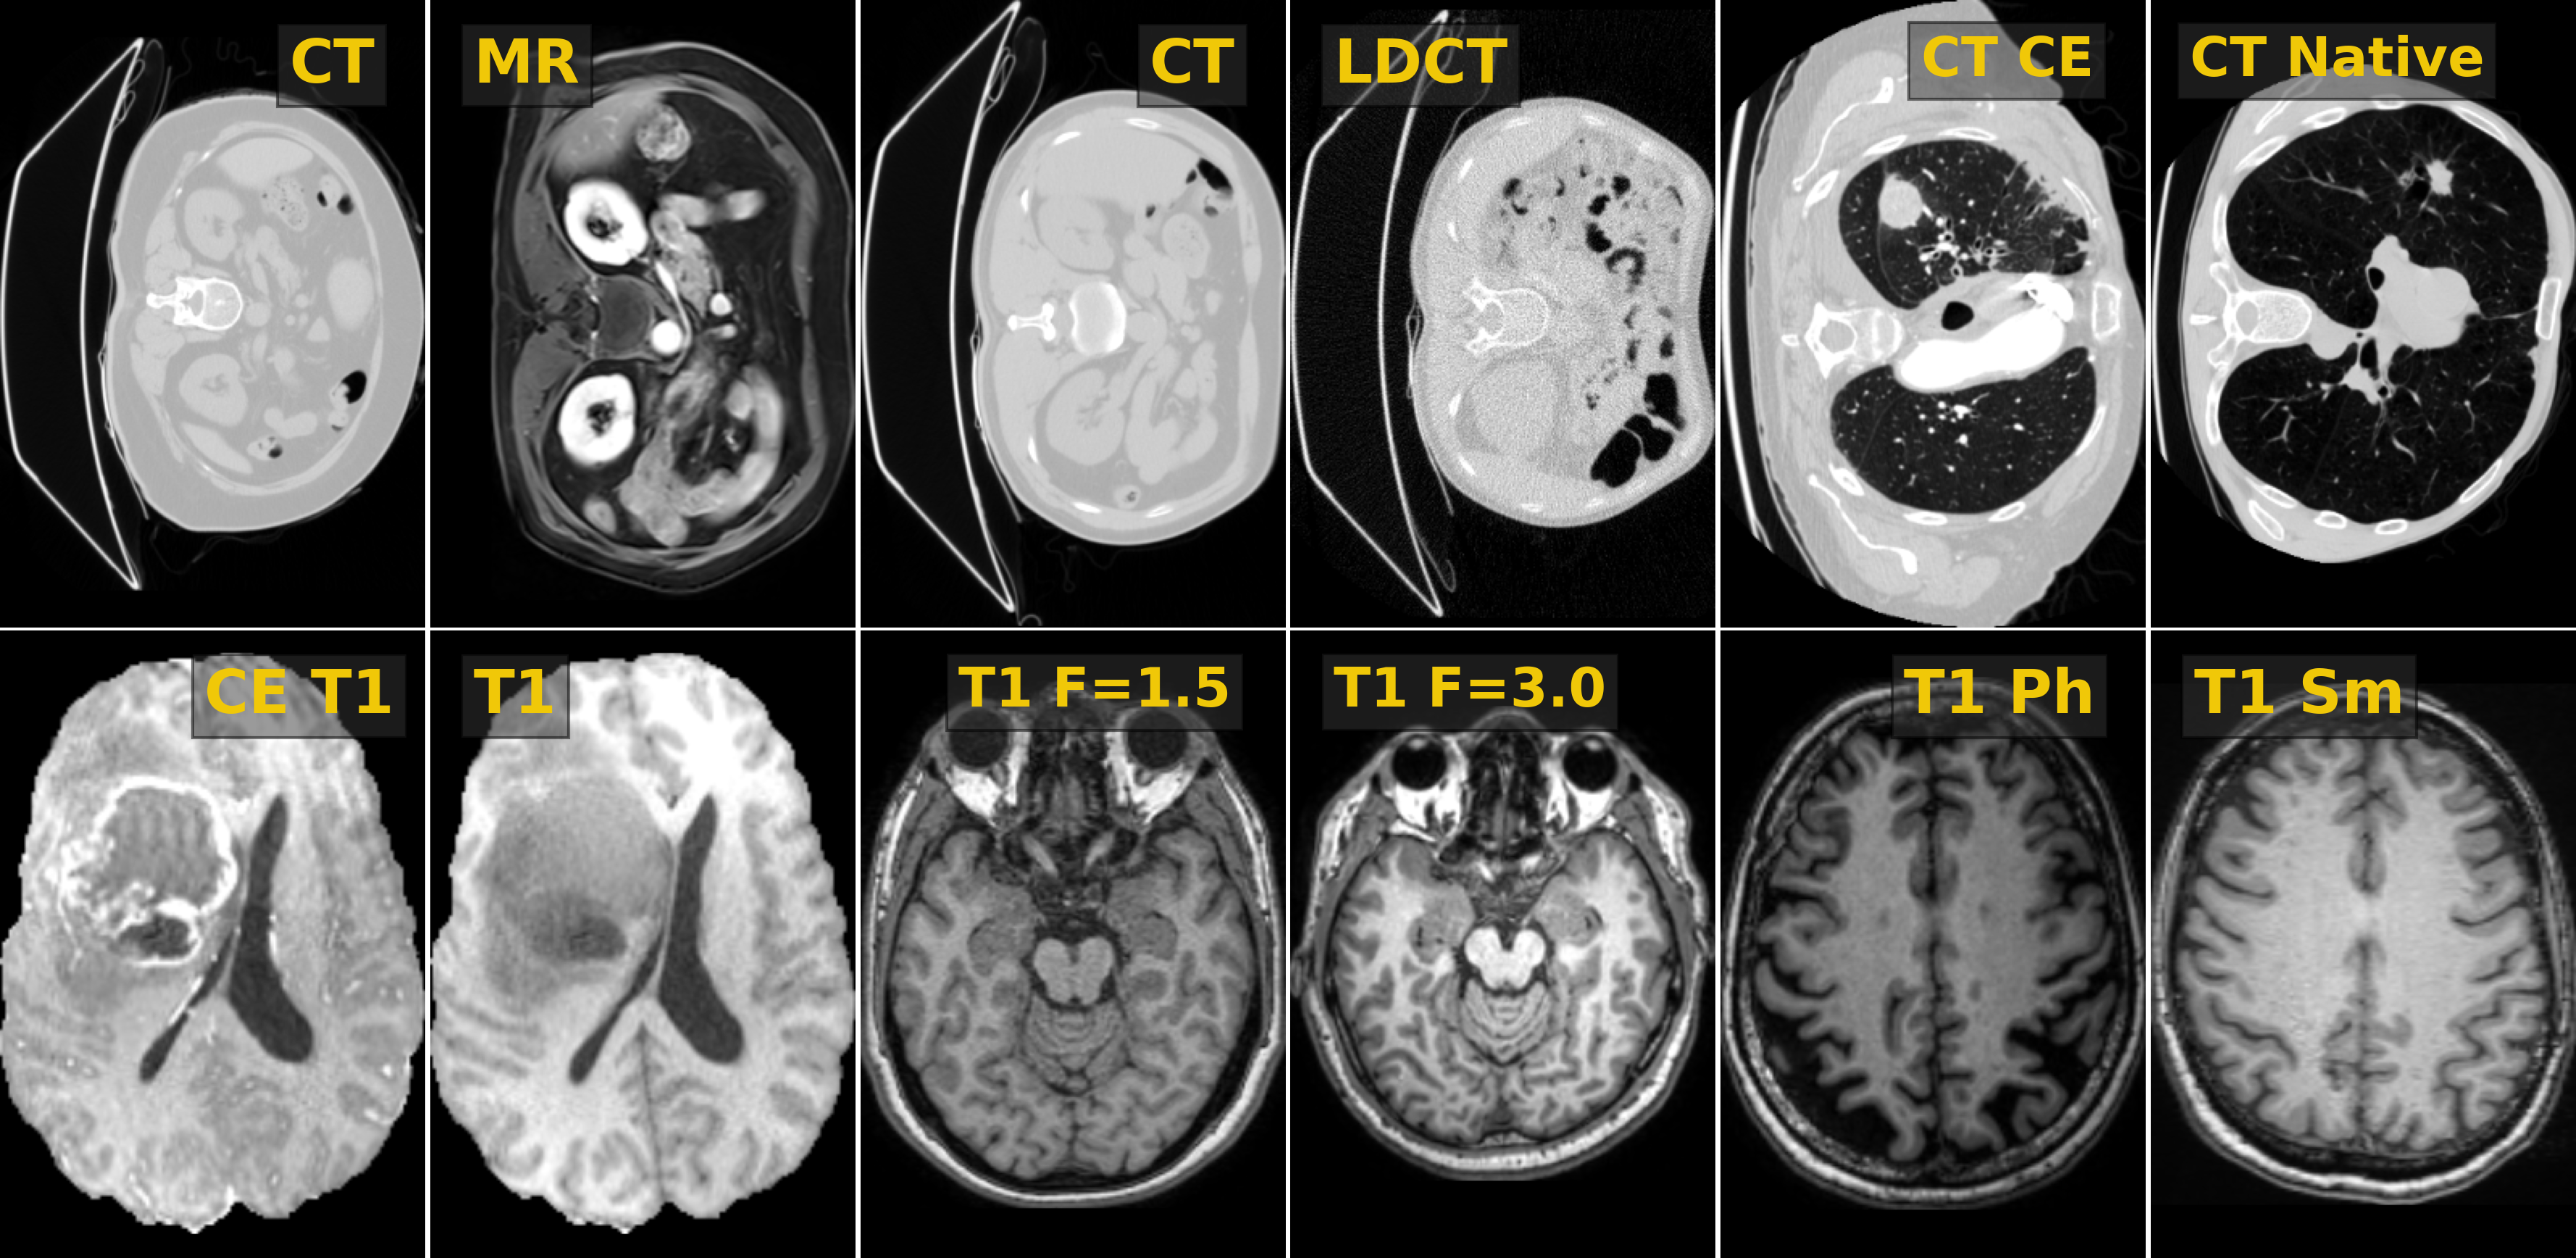
\includegraphics[width=1\linewidth]{Dissertation/Figures/4_da_bench/fig2_bench_examples.png}
%	\caption{Examples from individual domains in M3DA without segmentation masks for visual comparison between domains. Left to right, top to bottom: CT to MR, CT to LDCT, CT CE to CT native, CE T1 to T1, T1 Field (1.5T to 3T), T1 Scanner (Philips to Siemens).}
%	\label{fig:teaser2}
%\end{figure*}


\begin{landscape}
\begin{table}[p]
	\centering
	\caption{Main results on our benchmark in terms of multiclass average Dice score.}
	\label{tab:metrics_pure}

	%\resizebox{\linewidth}{!}{%
		\begin{tabular}{lcccccccccc}
			\toprule
			& MR$\ra$CT & CT$\ra$MR & LDCT & CE CT & T1 CE & T1 F & T1 Sc & T1 Mix & \textit{avg} & \textit{gap} \\
			
			\midrule
			
			Baseline & 0.03(0.04) & 0.03(0.04) & 0.13(0.16) & 0.23(0.27) & 0.43(0.17) & 0.74(0.07) & 0.77(0.03) & 0.56(0.16) & 0.365 & 0.0 \\
			
			\midrule
			
			SAM-Med & 0.02(0.01) & 0.04(0.03) & 0.52(0.12) & 0.41(0.31) & 0.27(0.15) & 0.65(0.08) & 0.76(0.04) & 0.49(0.27) & 0.394 & -1.0 \\
			
			UniModel & 0.03(0.02) & 0.01(0.01) & 0.25(0.19) & \textbf{0.47(0.31)} & 0.33(0.14) & 0.74(0.06) & 0.74(0.04) & 0.62(0.18) & 0.398 & 7.4 \\
			
			\midrule
			
			HM & 0.33(0.18) & 0.22(0.13) & 0.11(0.17) & 0.13(0.22) & 0.34(0.18) & 0.79(0.07) & 0.75(0.09) & 0.50(0.20) & 0.397 & -1.1 \\
			
			GAN3d & 0.33(0.13) & 0.26(0.11) & 0.33(0.17) & 0.13(0.20) & 0.34(0.17) & 0.79(0.04) & 0.71(0.02) & 0.76(0.02) & 0.458 & 9.5 \\
			
			MinEnt & 0.14(0.14) & 0.17(0.15) & 0.51(0.13) & 0.39(0.32) & 0.43(0.17) & 0.77(0.04) & 0.80(0.03) & 0.78(0.09) & 0.498 & 28.5 \\
			
			GAN2d & 0.20(0.15) & 0.41(0.14) & 0.53(0.19) & 0.22(0.26) & 0.40(0.18) & 0.85(0.01) & 0.80(0.03) & 0.80(0.02) & 0.525 & 30.2 \\
			
			GIN & \textbf{0.59(0.14)} & \textbf{0.64(0.10)} & 0.72(0.11) & 0.16(0.24) & 0.38(0.18) & 0.84(0.07) & 0.71(0.07) & 0.80(0.06) & 0.605 & 33.6 \\
			
			AdaBN & 0.32(0.16) & 0.35(0.18) & 0.59(0.20) & 0.29(0.29) & 0.43(0.17) & 0.78(0.04) & 0.83(0.02) & 0.80(0.06) & 0.550 & 35.0 \\
			
			DANN & 0.30(0.15) & 0.28(0.14) & 0.70(0.15) & 0.41(0.30) & 0.42(0.16) & 0.73(0.08) & 0.83(0.03) & 0.78(0.08) & 0.555 & 36.2 \\
			
			IN & 0.30(0.15) & 0.31(0.14) & 0.67(0.17) & 0.43(0.29) & 0.43(0.15) & 0.76(0.06) & 0.84(0.03) & 0.78(0.08) & 0.564 & 39.6 \\
			
			MIND & 0.56(0.17) & 0.59(0.12) & 0.24(0.15) & 0.42(0.24) & 0.34(0.16) & 0.86(0.04) & 0.87(0.04) & 0.84(0.03) & 0.590 & 45.9 \\
			
			Gamma & 0.35(0.18) & 0.17(0.15) & 0.24(0.23) & 0.44(0.31) & 0.44(0.16) & 0.89(0.02) & \textbf{0.91(0.01)} & 0.91(0.01) & 0.544 & 48.3 \\
			
			SE & 0.39(0.13) & 0.39(0.10) & 0.60(0.19) & 0.33(0.29) & 0.39(0.17) & 0.91(0.02) & 0.89(0.01) & \textbf{0.92(0.02)} & 0.602 & 51.7 \\
			
			nnAugm & 0.17(0.12) & 0.10(0.09) & \textbf{0.78(0.10)} & 0.39(0.32) & \textbf{0.45(0.16)} & \textbf{0.91(0.01)} & 0.90(0.01) & 0.89(0.01) & 0.573 & 51.9 \\
			
			\midrule
			
			Oracle & 0.84(0.09) & 0.83(0.04) & 0.81(0.10) & 0.52(0.30) & 0.69(0.18) & 0.95(0.02) & 0.96(0.01) & 0.96(0.01) & 0.820 & 100 \\
			
			\bottomrule
			
		\end{tabular}%}
	
\end{table}
\end{landscape}


%\begin{landscape}
%	\begin{table}[h]
%		\centering
%		\caption{Main results on our benchmark in terms of multiclass average Dice score.}
%		\label{tab:metrics_pure}
%		%\resizebox{\linewidth}{!}{%
%			\begin{tabular}{lcccccccccc}
%				\toprule
%				& MR$\rightarrow$CT & CT$\rightarrow$MR & CT$\rightarrow$ldCT & ceCT$\rightarrow$CT & T1ce$\rightarrow$T1 & T1 F & T1 Sc & T1 Mix & \textit{avg} & \textit{gap} \\
%				
%				\midrule
%				
%				Baseline & 0.03(0.04) & 0.03(0.04) & 0.13(0.16) & 0.23(0.27) & 0.43(0.17) & 0.74(0.07) & 0.77(0.03) & 0.56(0.16) & 0.365 & 0.0\% \\
%				
%				\midrule
%				
%				SAMMed & 0.02(0.01) & 0.04(0.03) & 0.52(0.12) & 0.41(0.31) & 0.27(0.15) & 0.65(0.08) & 0.76(0.04) & 0.49(0.27) & 0.394 & -1.0\% \\
%				
%				UniModel & 0.03(0.02) & 0.01(0.01) & 0.25(0.19) & \textbf{0.47(0.31)} & 0.33(0.14) & 0.74(0.06) & 0.74(0.04) & 0.62(0.18) & 0.398 & 7.4\% \\
%				
%				\midrule
%				
%				HM & 0.33(0.18) & 0.22(0.13) & 0.11(0.17) & 0.13(0.22) & 0.34(0.18) & 0.79(0.07) & 0.75(0.09) & 0.50(0.20) & 0.397 & -1.1\% \\
%				
%				cGAN3D & 0.33(0.13) & 0.26(0.11) & 0.33(0.17) & 0.13(0.20) & 0.34(0.17) & 0.79(0.04) & 0.71(0.02) & 0.76(0.02) & 0.458 & 9.5\% \\
%				
%				MinEnt & 0.14(0.14) & 0.17(0.15) & 0.51(0.13) & 0.39(0.32) & 0.43(0.17) & 0.77(0.04) & 0.80(0.03) & 0.78(0.09) & 0.498 & 28.5\% \\
%				
%				cGAN2D & 0.20(0.15) & 0.41(0.14) & 0.53(0.19) & 0.22(0.26) & 0.40(0.18) & 0.85(0.01) & 0.80(0.03) & 0.80(0.02) & 0.525 & 30.2\% \\
%				
%				GIN & \textbf{0.59(0.14)} & \textbf{0.64(0.10)} & 0.72(0.11) & 0.16(0.24) & 0.38(0.18) & 0.84(0.07) & 0.71(0.07) & 0.80(0.06) & 0.605 & 33.6\% \\
%				
%				AdaBN & 0.32(0.16) & 0.35(0.18) & 0.59(0.20) & 0.29(0.29) & 0.43(0.17) & 0.78(0.04) & 0.83(0.02) & 0.80(0.06) & 0.550 & 35.0\% \\
%				
%				DANN & 0.30(0.15) & 0.28(0.14) & 0.70(0.15) & 0.41(0.30) & 0.42(0.16) & 0.73(0.08) & 0.83(0.03) & 0.78(0.08) & 0.555 & 36.2\% \\
%				
%				IN & 0.30(0.15) & 0.31(0.14) & 0.67(0.17) & 0.43(0.29) & 0.43(0.15) & 0.76(0.06) & 0.84(0.03) & 0.78(0.08) & 0.564 & 39.6\% \\
%				
%				MIND & 0.56(0.17) & 0.59(0.12) & 0.24(0.15) & 0.42(0.24) & 0.34(0.16) & 0.86(0.04) & 0.87(0.04) & 0.84(0.03) & 0.590 & 45.9\% \\
%				
%				Gamma & 0.35(0.18) & 0.17(0.15) & 0.24(0.23) & 0.44(0.31) & 0.44(0.16) & 0.89(0.02) & \textbf{0.91(0.01)} & 0.91(0.01) & 0.544 & 48.3\% \\
%				
%				SE & 0.39(0.13) & 0.39(0.10) & 0.60(0.19) & 0.33(0.29) & 0.39(0.17) & 0.91(0.02) & 0.89(0.01) & \textbf{0.92(0.02)} & 0.602 & 51.7\% \\
%				
%				nnAugm & 0.17(0.12) & 0.10(0.09) & \textbf{0.78(0.10)} & 0.39(0.32) & \textbf{0.45(0.16)} & \textbf{0.91(0.01)} & 0.90(0.01) & 0.89(0.01) & 0.573 & 51.9\% \\
%				
%				\midrule
%				
%				Oracle        & 0.84(0.09) & 0.83(0.04) & 0.81(0.10) & 0.52(0.30) & 0.69(0.18) & 0.95(0.02) & 0.96(0.01) & 0.96(0.01) & 0.820 & 100\% \\
%				
%				\bottomrule
%				
%			\end{tabular}%}
%		
%	\end{table}
%\end{landscape}





\begin{landscape}
\begin{table}[p]
	\centering
	\caption{Performance gain of different methods supplemented with nnU-Net augmentations.}
	
	%\resizebox{\linewidth}{!}{%
		\begin{tabular}{lcccccccccc}
			\toprule
			& MR$\ra$CT & CT$\ra$MR & LDCT & CE CT & T1 CE & T1 F & T1 Sc & T1 Mix & \textit{avg DSC} & \textit{gap (\%)} \\
			
			\midrule
			
			CycleGAN 3D & $\uparrow$0.031 & $\uparrow$0.200 & $\uparrow$0.353 & $\uparrow$0.091 & $\uparrow$0.034 & $\uparrow$0.034 & $\uparrow$0.097 & $\uparrow$0.017 & $\uparrow$0.107 & 34.1 $\uparrow$24.6 \\
			
			CycleGAN 2D & $\uparrow$0.096 & $\uparrow$0.055 & $\uparrow$0.136 & $\uparrow$0.117 & $\uparrow$0.018 & $\uparrow$0.013 & $\uparrow$0.049 & $\uparrow$0.020 & $\uparrow$0.063 & 45.5 $\uparrow$15.3 \\
			
			Baseline & $\uparrow$0.134 & $\uparrow$0.070 & $\uparrow$0.646 & $\uparrow$0.164 & $\uparrow$0.020 & $\uparrow$0.169 & $\uparrow$0.131 & $\uparrow$0.329 & $\uparrow$0.208 & 51.9 $\uparrow$51.9 \\
			
			DANN        & $\uparrow$0.118 & $\uparrow$0.071 & $\uparrow$0.110 & $\uparrow$0.002 & $\downarrow$-0.013 & $\uparrow$0.169 & $\uparrow$0.015 & $\uparrow$0.109 & $\uparrow$0.072 & 54.9 $\uparrow$23.3 \\
			
			IN          & $\uparrow$0.119 & $\uparrow$0.163 & $\uparrow$0.128 & $\downarrow$-0.017 & $\downarrow$-0.012 & $\uparrow$0.151 & $\uparrow$0.016 & $\uparrow$0.099 & $\uparrow$0.081 & 58.1 $\uparrow$26.6 \\
			
			AdaBN       & $\uparrow$0.173 & $\uparrow$0.179 & $\uparrow$0.017 & $\uparrow$0.070 & $\uparrow$0.021 & $\uparrow$0.129 & $\uparrow$0.057 & $\uparrow$0.096 & $\uparrow$0.092 & 59.2 $\uparrow$24.2 \\
			
			SE          & $\uparrow$0.068 & $\uparrow$0.183 & $\uparrow$0.165 & $\uparrow$0.057 & $\downarrow$-0.014 & $\downarrow$-0.004 & $\uparrow$0.014 & $\downarrow$-0.030 & $\uparrow$0.055 & 60.1 \enspace $\uparrow$8.4 \\
			
			MinEnt      & $\uparrow$0.248 & $\uparrow$0.190 & $\uparrow$0.283 & $\uparrow$0.057 & $\uparrow$0.019 & $\uparrow$0.133 & $\uparrow$0.103 & $\uparrow$0.116 & $\uparrow$0.143 & \textbf{62.0} $\uparrow$33.5 \\
			
			\midrule
			
			\textit{average} &$\uparrow$0.123 & $\uparrow$0.139 & $\uparrow$0.230 & $\uparrow$0.068 & $\uparrow$0.009 & $\uparrow$0.099 & $\uparrow$0.060 & $\uparrow$0.095 & $\uparrow$0.103 & $\uparrow$26.0 \\  % 53.2\%
			
			\bottomrule
	\end{tabular}%}
	\label{tab:ablation_aug}
\end{table}
\end{landscape}


To support research under highly realistic clinical conditions, the chapter also presents the Burdenko’s Glioblastoma Progression (BGP) dataset. The BGP dataset contains MRI studies from 180 glioblastoma patients acquired for radiotherapy planning, with images sourced from four different scanner vendors and spanning diverse acquisition protocols. This allows researchers to test the generalization of models under in-the-wild domain shifts where the target domain is not fully known or controlled.

In summary, this chapter contributes a rigorous benchmarking suite for DA in 3D medical imaging and reveals key limitations of current approaches. It motivates future work on methods that can adapt effectively across multiple axes of variability without relying on restrictive assumptions about the target domain.


% %%%%%%%%%%%%%%% CHAPTER 4 %%%%%%%%%%%%%%%


The fourth chapter, \textbf{Benchmark for OOD in 3D Medical Image Segmentation}, addresses the critical challenge of out-of-distribution (OOD) detection in clinical deployment of segmentation models. While previous chapters focused on adapting models to known domain shifts, this chapter explores the complementary task of identifying when input data deviates significantly from the training distribution -- a prerequisite for safe model application in real-world medical environments.

To systematically investigate this problem, the chapter introduces a dedicated benchmark for OOD detection in 3D medical image segmentation. The benchmark is designed around multiple clinically relevant use cases, where segmentation models are applied to samples that violate assumptions about modality, anatomy, or acquisition settings. These include acquisition protocol, patient population, and anatomical region changes and imaging artifact encounter in both CT and MRI modalities.

%(Figure~\ref{fig:ct})
%(Figure~\ref{fig:mri})

%\begin{figure}[h]
%	\centering
%	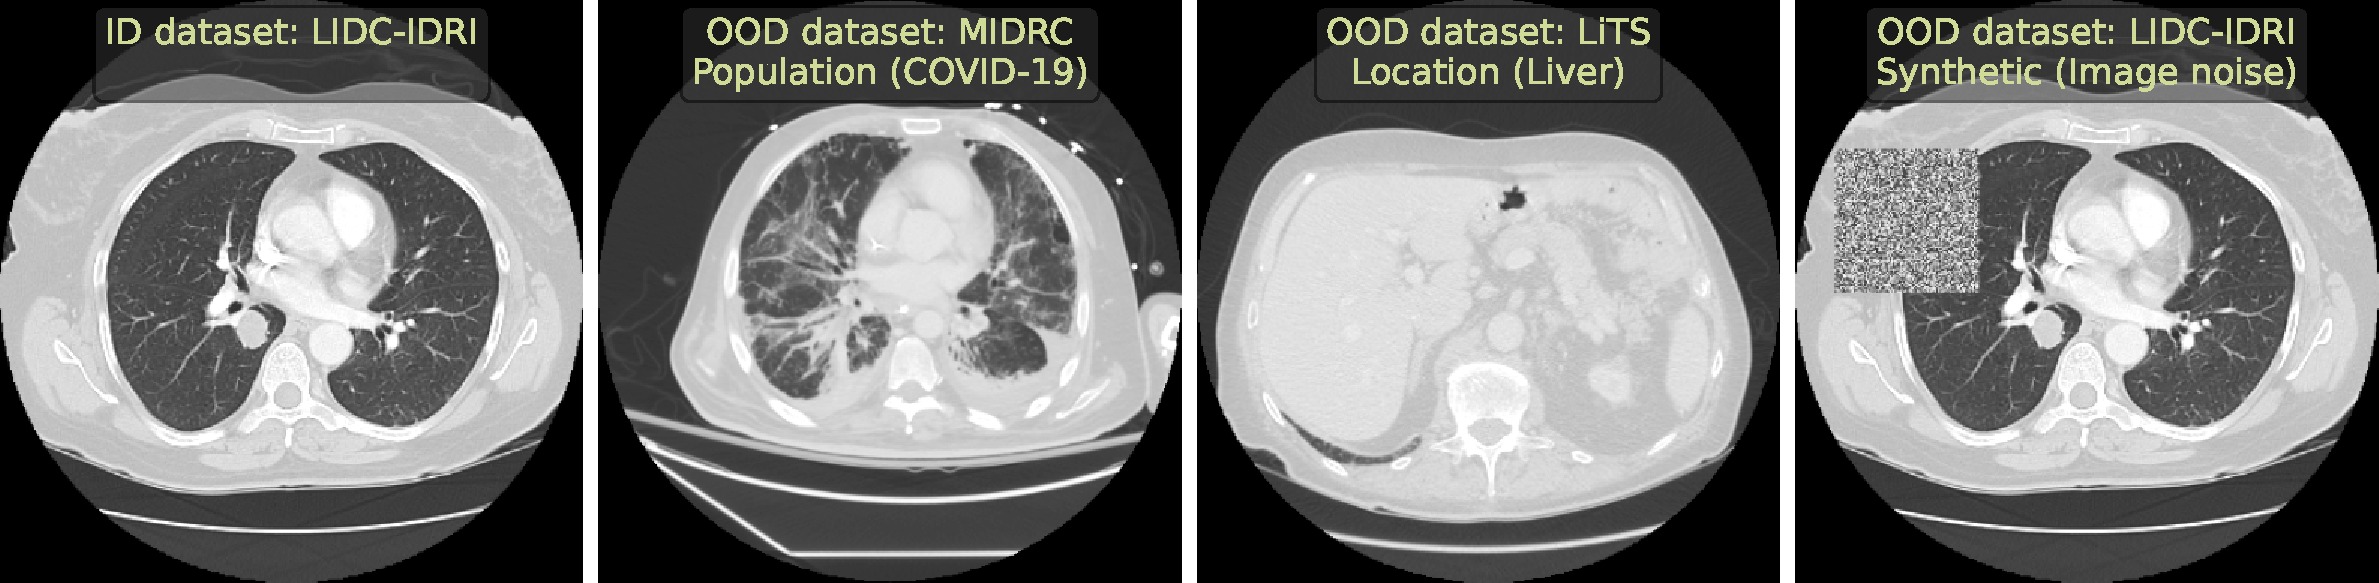
\includegraphics[width=\textwidth]{Dissertation/Figures/5_ood_bench/ct_examples_2.pdf}
%	\caption{Examples of CT images (representative axial slices) from different simulated OOD sources in our benchmark.}
%	\label{fig:ct}
%\end{figure}
%
%\begin{figure}[h]
%	\centering
%	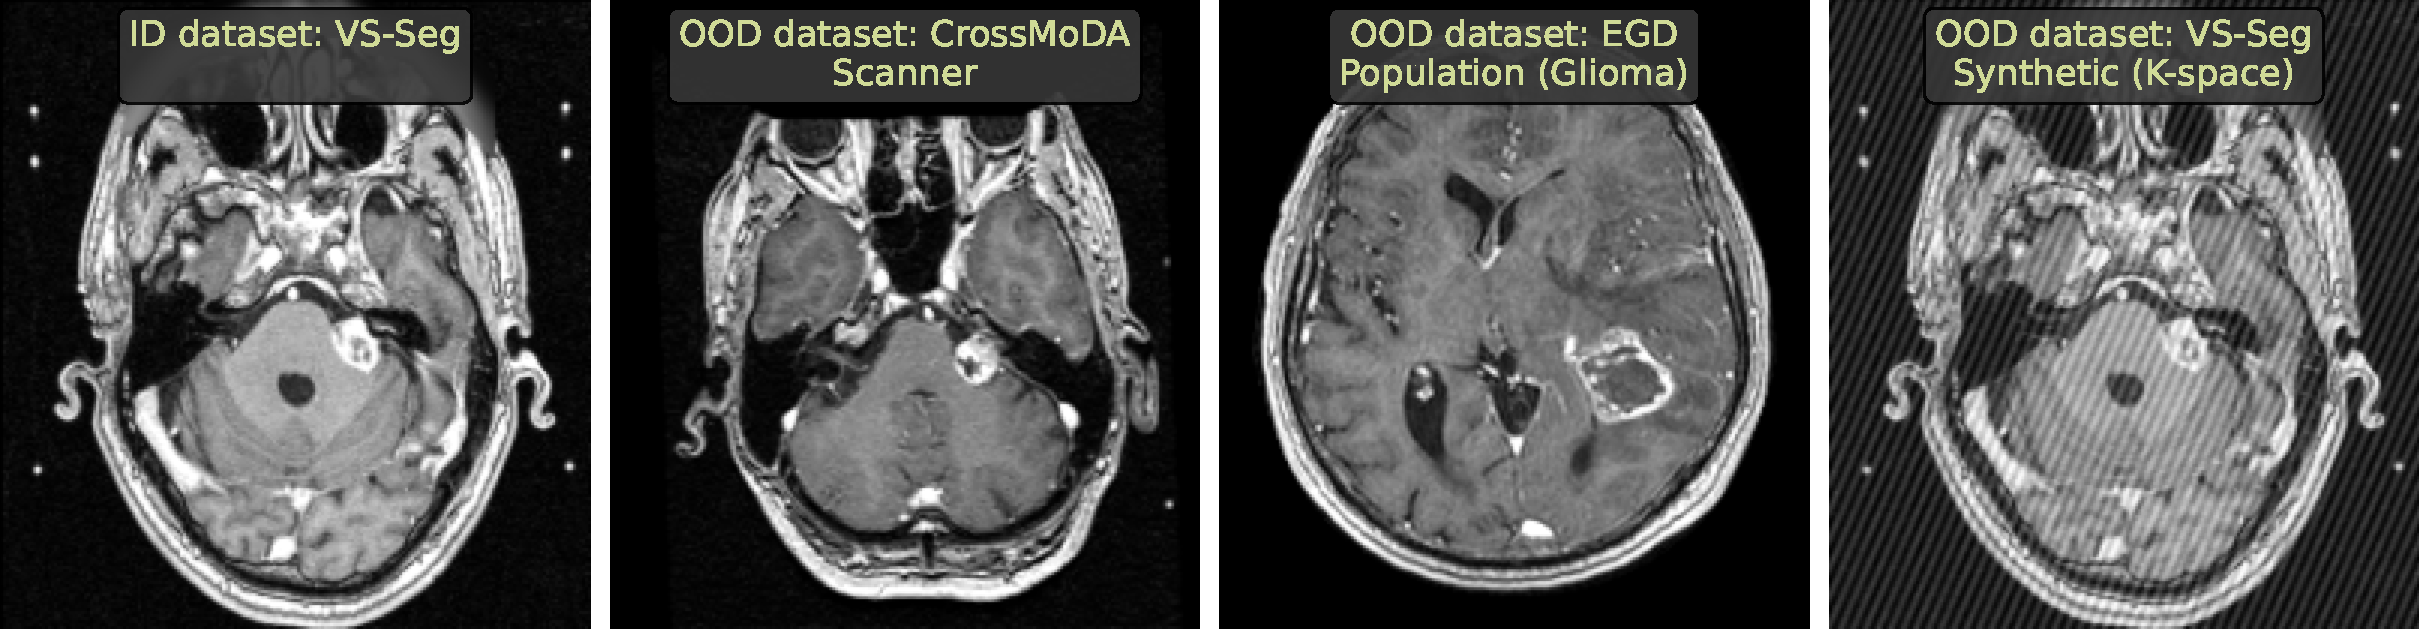
\includegraphics[width=\textwidth]{Dissertation/Figures/5_ood_bench/mri_examples_2.pdf}
%	\caption{Examples of MRI images (representative axial slices) from different simulated OOD sources in our benchmark.}
%	\label{fig:mri}
%\end{figure}

The chapter evaluates several state-of-the-art OOD detection methods, including softmax-based confidence scores, Monte-Carlo dropout, and self-supervised approaches. Despite their success in 2D natural image tasks, most methods exhibit poor performance in the 3D medical setting, with high false positive rates.% (Table~\ref{tab:res_fpr}).

To complement these baselines, the chapter proposes a novel lightweight method, Intensity Histogram Features (IHF), which captures global image statistics using simple summary histograms of voxel intensities. As SpotTUnet-based analysis suggests, the earlier network's layers contain the most domain-specific information. Taking this analysis to the extreme, we hypothesize that we can extract enough domain-specific information directly from the image (i.e., the zeroth network's layer). A histogram is a convenient way to do so.

We schematically present our method, called Intensity Histogram Features (IHF), in Figure~\ref{fig:ihf}. It consists of three steps: (1) calculating intensity histograms of images and using them as vectors, (2) reducing their dimensionality with PCA, and (3) running an outlier detection algorithm on these vectors.

\begin{landscape}
	\begin{figure}[p]
		\centering
		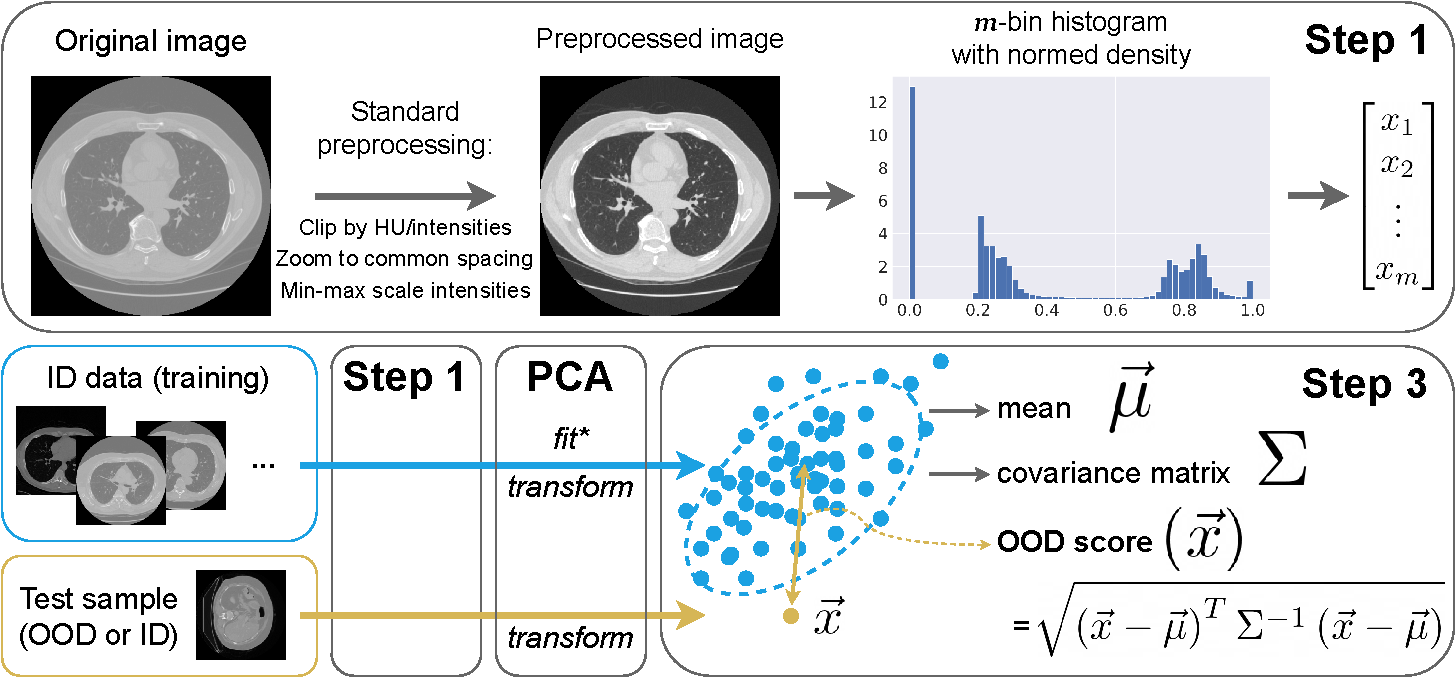
\includegraphics[width=\linewidth]{Dissertation/Figures/5_ood_bench/method-1.pdf}
		\caption{The proposed OOD detection method, called \textit{Intensity Histogram Features (IHF)}.}
		\label{fig:ihf}
	\end{figure}
\end{landscape}

Step 1: preprocessing and histograms. All images undergo the same preprocessing pipeline to standardize the intensity distribution. Given a preprocessed image $x$, we compute a probability density function of its intensities in $m$ bins, a histogram $e(x) \in \mathbb{R}^m$, and further use these vectors $e(x)$.
	
Step 2: Principal Component Analysis (PCA). As an optional step, we use PCA~\cite{pca} to reduce the dimensions $m$. The main reason to use it is that some outlier detection algorithms at Step 3 behave unstable in high dimensional spaces. For instance, calculating Mahalanobis distance requires reversing the empirical sample covariance matrix, and this matrix is likely to become ill-conditioned or singular with larger $m$. We fit PCA$_v$ once on the training data $E_{tr}$ to preserve $v = 99.99\%$ of the explained variance. This way, we eliminate the potential instability and preserve the distribution properties. $E_{tr}$ consists of row-vectors $e(x_{tr})$ for all training images $x_{tr} \in X_{tr}$. Further, we use transformed vectors $\tilde{e}(x) = \text{PCA}_v (e(x))$.
	
Step 3: OOD detection algorithm. To calculate an OOD score for $x$, we can apply any distance- or density-based outlier detection method. As our first approach, we can calculate Mahalanobis distance $S_{Mah}(x)$:

\begin{equation}
	\label{eq:mah}
	S_{Mah}(x) = \sqrt{ \left( \tilde{e}(x) - \hat{\mu} \right)^T \hat{\Sigma}^{-1} \left( \tilde{e}(x) - \hat{\mu} \right) },
\end{equation}

\noindent
where $\hat{\mu}$ and $\hat{\Sigma}$ are the estimated mean and covariance matrix on the training set, $\hat{\mu} = \frac{1}{|X_{tr}|} \sum_{x_{tr} \in X_{tr}} \tilde{e} \left(x_{tr}\right)$ and $\hat{\Sigma} = \frac{1}{|X_{tr}|} \sum_{x_{tr} \in X_{tr}} \left( \tilde{e} (x_{tr}) - \hat{\mu} \right) \left( \tilde{e} (x_{tr}) - \hat{\mu} \right)^T$.

Alternatively, one can calculate the distance to the nearest neighbor (min-distance) $S_{NN}(x)$:

\begin{equation}
	\label{eq:nn}
	S_{NN}(x) = \min_{x_{tr} \in X_{tr}} || \tilde{e} (x) - \tilde{e} (x_{tr}) ||_2.
\end{equation}

Using $S_{Mah}$ (Equation~\ref{eq:mah}) and $S_{NN}$ (Equation~\ref{eq:nn}) corresponds to the methods IHF-Mah and IHF-NN, respectively. We included them in our experiments independently.

Despite its simplicity, IHF achieves competitive performance: ranking top-1 in multiple benchmark scenarios (Table~\ref{tab:res_fpr}) and ranked the top-2 solution in the Medical Out-of-Distribution Challenge (MOOD) in both 2022 and 2023~\cite{zimmerer2022mood}. The method’s efficiency and interpretability make it a strong candidate for integration into clinical pipelines.



\begin{table}[h]
	\centering
	\caption{Comparison of the considered OOD detection methods in terms of FPR@TPR95\% scores (lower is better). We highlight the best scores in every row in \textbf{bold} and ranked the methods by their average performance. The first and second sections correspond to CT and MRI setups, respectively.}
	\resizebox{\textwidth}{!}{%
		\begin{tabular}{llllllllll}
			\toprule
			\textbf{OOD Setup} &            \textbf{IHF-NN} &             \textbf{SVD} &             \textbf{IHF-Mah} &      \textbf{MOOD-1} &           \textbf{G-ODIN} &             \textbf{Volume} &   \textbf{MCD} & \textbf{Ensemble} &   \textbf{Entropy} \\
			\midrule
			Location (Head)           &  \textbf{0.00}  &  \textbf{0.00}  &  \textbf{0.00}  &            0.12 &            0.55 &            0.53 &  0.36 &     0.51 &  0.56 \\
			Location (Liver)          &            0.51 &  \textbf{0.13}  &            0.64 &            0.56 &            0.56 &            0.84 &  0.89 &     0.93 &  0.78 \\
			Population (COVID-19)     &            0.54 &            0.75 &            0.72 &  \textbf{0.51}  &            0.54 &            0.82 &  0.58 &     0.58 &  0.87 \\
			Scanner                 &            0.88 &            0.89 &            0.85 &  \textbf{0.73}  &            0.92 &            0.86 &  0.89 &     0.90 &  0.83 \\
			Synthetic (Elastic)       &  \textbf{0.15}  &            0.37 &            0.67 &            0.16 &            0.59 &            0.81 &  0.42 &     0.37 &  0.84 \\
			Synthetic (Image noise)  &            0.49 &            0.37 &            0.62 &  \textbf{0.11}  &            0.89 &            0.85 &  0.87 &     0.82 &  0.81 \\
			\midrule
			Population (Glioblastoma) &  \textbf{0.00}  &  \textbf{0.00}  &  \textbf{0.00}  &            0.10 &            0.21 &            0.01 &  0.85 &     0.81 &  0.86 \\
			Population (Healthy)      &  \textbf{0.00}  &  \textbf{0.00}  &  \textbf{0.00}  &            0.11 &  \textbf{0.00}  &  \textbf{0.00}  &  0.88 &     10.0 &  0.85 \\
			Scanner                   &  \textbf{0.00}  &  \textbf{0.00}  &  \textbf{0.00}  &            0.15 &  \textbf{0.00}  &            0.74 &  0.63 &     0.66 &  0.89 \\
			Synthetic (K-space noise) &  \textbf{0.00}  &            0.36 &  \textbf{0.00}  &            0.88 &            0.88 &            0.90 &  0.82 &     0.77 &  0.73 \\
			Synthetic (Anisotropy)    &            0.09 &            0.20 &  \textbf{0.05}  &            0.57 &            0.88 &            0.93 &  0.77 &     0.77 &  0.81 \\
			Synthetic (Motion)        &  \textbf{0.00}  &            0.58 &  \textbf{0.00}  &            0.73 &            0.93 &            0.94 &  0.85 &     0.88 &  0.91 \\
			Synthetic (Image noise)   &            0.47 &            0.33 &            0.47 &  \textbf{0.30}  &            0.56 &            0.71 &  0.78 &     0.75 &  0.75 \\
			\midrule
			CT average                &            0.43 &            0.42 &            0.58 &  \textbf{0.36}  &            0.67 &            0.79 &  0.67 &     0.68 &  0.78 \\
			MRI average               &            0.08 &            0.21 &  \textbf{0.07}  &            0.41 &            0.50 &            0.60 &  0.80 &     0.81 &  0.83 \\
			\bottomrule
	\end{tabular}}
	\label{tab:res_fpr}
\end{table}


In summary, this chapter reveals the limitations of current OOD detection methods in 3D medical image segmentation, provides a standardized evaluation framework and a strong OOD detection baseline for future research. Together with previous chapters, it contributes to the broader goal of building safe, adaptive, and deployable AI systems for medical imaging.


% %%%%%%%%%%%%%%% CONCLUSION %%%%%%%%%%%%%%

The last chapter, \textbf{Conclusion}, summarizes the results and discusses future work.

% The \textbf{conclusions chapter} summarizes the thesis, consolidates the presented results, and offers a concise summary of the investigation’s significance

\section*{Conclusion}

This dissertation is devoted to the development of mathematically grounded and practically robust deep learning methods for domain adaptation and out-of-distribution detection in 3D medical image segmentation. The work systematically addresses the challenge of domain shift, which remains a critical obstacle to the reliable deployment of machine learning systems in clinical environments.

\begin{enumerate}
	
	\item A gradient-based supervised domain adaptation method, SpotTUnet, was proposed to address the problem of layer-wise adaptation in convolutional neural networks for medical image segmentation. The method optimizes a learnable layer selection policy, allowing to fine-tune the most shift-sensitive layers. The effectiveness of this approach was confirmed through extensive experimental validation, including statistically significant improvements over common fine-tuning baselines in few-shot adaptation scenarios. From a practical standpoint, SpotTUnet provides interpretable visualizations of domain shift sensitivity across network layers, which we further used to guide the design of F-Consistency and to enhance performance of existing DA algorithms, such as DANN~\cite{dann}, on the M3DA benchmark. Moreover, conclusions drawn from SpotTUnet contributed to the development of the IHF method for out-of-distribution detection. The proposed approach can be further extended to unsupervised setting by leveraging auxiliary domain shift criteria and emerging transformer-based architectures~\cite{unetr}.
        
    \item Two complementary DA methods were proposed to address performance degradation in CT segmentation caused by variations in reconstruction kernels. First, a knowledge-driven augmentation technique, Filtered Back-Projection Augmentation (FBPAug), was developed to simulate such kernel-induced domain shifts by modeling the mathematics of CT image formation in sinogram space. Second, a data-driven unsupervised DA method, F-Consistency, was introduced to align internal network representations of paired CT images reconstructed with different kernels. Both methods demonstrated statistically significant improvements over state-of-the-art approaches: FBPAug achieved high consistency in the zero-shot adaptation setting, while F-Consistency further increased segmentation quality in the standard unsupervised DA setting. FBPAug has been integrated into the production pipeline of a medical imaging startup, where it significantly improved the robustness and accuracy of CT-based segmentation models used in clinical practice. Further research may focus on combining FBPAug-generated pseudo-pairs with the F-Consistency objective in a self-supervised learning framework to obtain even more robust pretrained foundational model.
    
    \item A large-scale benchmark, M3DA, was developed to evaluate unsupervised DA methods in 3D medical image segmentation under realistic and diverse shift scenarios. The benchmark reveals that existing methods close only 62\% of the performance gap on average. To support clinical relevance, a new multi-modal dataset, BGP, was published for glioblastoma segmentation with high intra-institution variability. These contributions enable systematic comparison of methods and guide the design of robust and generalizable DA algorithms.
    
    \item A benchmark for OOD detection in 3D medical segmentation was constructed, including clinically relevant scenarios, and was used to identify fundamental limitations of current methods. A lightweight method, IHF, was proposed as an interpretable and computationally efficient baseline, achieving top-2 in the MOOD 2022 and 2023 challenges. The benchmark and IHF serve as a foundation for further theoretical study of distributional uncertainty in medical imaging data.
    
\end{enumerate}

The results and insights of this dissertation have already served as a foundation for several subsequent scientific works. Firstly, we used the proposed OOD benchmark to develop a novel OOD detection metric and theoretically justified framework~\cite{vasiliuk2023redesigning}. We also used components of this benchmark to analyze predictive uncertainty at the level of distinct predicted components~\cite{vasiliuk2022exploring}. Finally, the authors of~\cite{goncharov2023vox2vec}, integrated FBPAug into a self-supervised learning framework, realizing a direction for augmentation that was originally suggested in this dissertation. These works demonstrate the relevance of the presented contributions and point toward continued progress in the robust deployment of deep learning in medical imaging.
